\documentclass[a4paper,11pt]{report}
\usepackage{chuan_math_gkt}
\usetikzlibrary{angles,quotes,intersections,patterns,decorations.pathreplacing}
\chuanexamsetup

\begin{document}
\examfontsize

\examsecret{绝密$\bigstar$启用前}

\examtitle{2022年普通高等学校招生全国统一考试（北京卷）}{数\quad 学}

\noticetitle
\begin{examnotice}
\item 答卷前，考生务必将自己的姓名、准考证号填写在答题卡上。
\item 回答选择题时，选出每小题的答案后，用铅笔把答题卡上对应题目的答案标号涂黑。如需改动，用橡皮擦干净后，再选涂其他答案标号。回答非选择题时，将答案写在答题卡上。写在本试卷上无效。
\item 考试结束后，将本试卷和答题卡一并交回。
\end{examnotice}


\examsection{一、选择题：本题共10小题，每小题4分，共40分。在每小题给出的四个选项中，只有一项是符合题目要求的。}
\begin{examquestions}
\item 已知全集 $U=\{x\mid -3<x<3\}$，集合 $A=\{x\mid -2<x\leq1\}$，则 $\complement_U A=$
\fourchoices{$(-2,1]$}{$(-3,-2)\cup[1,3)$}{$[-2,1)$}{$(-3,-2]\cup(1,3)$}
\item 若复数 $z$ 满足 $\mathrm{i}z=3-4\mathrm{i}$，则 $|z|=$
\fourchoices{$1$}{$5$}{$7$}{$25$}
\item 若直线 $2x+y-1=0$ 是圆 $(x-a)^2+y^2=1$ 的一条对称轴，则 $a=$
\fourchoices{\tallchoice{$\dfrac12$}}{$-\dfrac12$}{$1$}{$-1$}
\item 已知函数 $f(x)=\dfrac{1}{1+2^x}$，则对任意实数 $x$，有
\twochoices{$f(-x)+f(x)=0$}{$f(-x)-f(x)=0$}{$f(-x)+f(x)=1$}{$f(-x)-f(x)=\dfrac13$}
\item 已知函数 $f(x)=\cos^2x-\sin^2x$，则
\twochoices{\tallchoice{$f(x)$ 在 $\left(-\dfrac\pi2,-\dfrac\pi6\right)$ 上单调递减}}{$f(x)$ 在 $\left(-\dfrac\pi4,\dfrac\pi{12}\right)$ 上单调递增}{\tallchoice{$f(x)$ 在 $\left(0,\dfrac\pi3\right)$ 上单调递减}}{$f(x)$ 在 $\left(\dfrac\pi4,\dfrac{7\pi}{12}\right)$ 上单调递增}
\item 设 $\{a_n\}$ 是公差不为 $0$ 的无穷等差数列，则“$\{a_n\}$ 为递增数列”是“存在正整数 $N_0$，当 $n>N_0$ 时，$a_n>0$”的
\twochoices{充分而不必要条件}{必要而不充分条件}{充分必要条件}{既不充分也不必要条件}
\item 在北京冬奥会上，国家速滑馆“冰丝带”使用高效环保的二氧化碳跨临界直冷制冰技术，为实现绿色冬奥作出了贡献. 如图描述了一定条件下二氧化碳所处的状态与 $T$ 和 $\lg P$ 的关系，其中 $T$ 表示温度，单位是 $\mathrm K$；$P$ 表示压强，单位是 $\mathrm{bar}$. 下列结论中正确的是
\begin{tightcenter}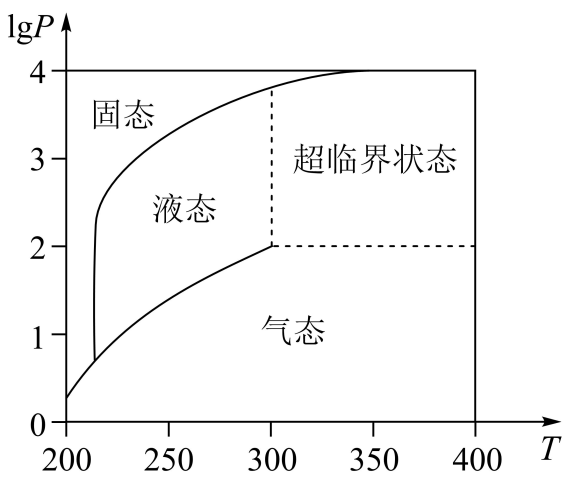
\includegraphics[width=5.0cm]{figures/2022_bj_q7.png}\end{tightcenter}
\onechoices{当 $T=220$，$P=1026$ 时，二氧化碳处于液态}{当 $T=270$，$P=128$ 时，二氧化碳处于气态}{当 $T=300$，$P=9987$ 时，二氧化碳处于超临界状态}{当 $T=360$，$P=729$ 时，二氧化碳处于超临界状态}
\item 若 $(2x-1)^4=a_4x^4+a_3x^3+a_2x^2+a_1x+a_0$，则 $a_0+a_2+a_4=$
\fourchoices{$40$}{$41$}{$-40$}{$-41$}
\item 已知正三棱锥 $P-ABC$ 的六条棱长均为 $6$，$S$ 是 $\triangle ABC$ 及其内部的点构成的集合. 设集合 $T=\{Q\in S\mid PQ\leq5\}$，则 $T$ 表示的区域的面积为
\fourchoices{$\dfrac{3\pi}{4}$}{$\pi$}{$2\pi$}{$3\pi$}
\item 在 $\triangle ABC$ 中，$AC=3$，$BC=4$，$\angle C=90^\circ$. $P$ 为 $\triangle ABC$ 所在平面内的动点，且 $PC=1$，则 $\vec{PA}\cdot\vec{PB}$ 的取值范围是
\fourchoices{$[-5,3]$}{$[-3,5]$}{$[-6,4]$}{$[-4,6]$}
\end{examquestions}

\examsection{二、填空题：本题共5小题，每小题5分，共25分。}
\begin{examquestions}[start=11]
\item 函数 $f(x)=\dfrac1x+\sqrt{1-x}$ 的定义域是\blank.
\item 已知双曲线 $y^2+\dfrac{x^2}{m}=1$ 的渐近线方程为 $y=\pm\dfrac{\sqrt3}{3}x$，则 $m=$\blank.
\item 若函数 $f(x)=A\sin x-\sqrt3\cos x$ 的一个零点为 $\dfrac\pi3$，则 $A=$\blank；$f\left(\dfrac\pi{12}\right)=$\blank.
\item 设函数 $f(x)=\linsys{-ax+1,\quad x<a,\\(x-2)^2,\quad x\geq a}$，若 $f(x)$ 存在最小值，则 $a$ 的一个取值为\blank；$a$ 的最大值为\blank.
\newpage
\item 已知数列 $\{a_n\}$ 各项均为正数，其前 $n$ 项和 $S_n$ 满足 $a_nS_n=9(n=1,2,\cdots)$. 给出下列四个结论：①$\{a_n\}$ 的第 $2$ 项小于 $3$；②$\{a_n\}$ 为等比数列；③$\{a_n\}$ 为递减数列；④$\{a_n\}$ 中存在小于 $\dfrac1{100}$ 的项. 其中所有正确结论的序号是\blank.
\end{examquestions}

\examsection{三、解答题：本题共6小题，共85分。解答应写出文字说明、证明过程或演算步骤。}
\begin{examanswers}[start=16]
\item（13分）

在 $\triangle ABC$ 中，$\sin2C=\sqrt3\sin C$.

（1）求 $\angle C$；

（2）若 $b=6$，且 $\triangle ABC$ 的面积为 $6\sqrt3$，求 $\triangle ABC$ 的周长.
\item（13分）

如图，在三棱柱 $ABC-A_1B_1C_1$ 中，侧面 $BCC_1B_1$ 为正方形，平面 $BCC_1B_1\perp$ 平面 $ABB_1A_1$，$AB=BC=2$，$M,N$ 分别为 $A_1B_1,AC$ 的中点.

\noindent\begin{minipage}[t]{0.62\linewidth}
（1）求证：$MN\parallel$ 平面 $BCC_1B_1$；

（2）再从条件①、条件②这两个条件中选择一个作为已知，求直线 $AB$ 与平面 $BMN$ 所成角的正弦值.

{\center{条件①：$AB\perp MN$；条件②：$BM=MN$.}}

（注：如果选择条件①和条件②分别解答，按第一个解答计分.）
\end{minipage}\hfill
\begin{minipage}[t]{0.31\linewidth}
\vspace{-1em}\centering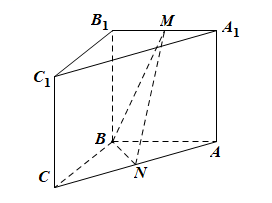
\includegraphics[width=\linewidth]{figures/2022_bj_q17.png}
\end{minipage}
\item（14分）

在校运动会上，只有甲、乙、丙三名同学参加铅球比赛，比赛成绩达到 $9.50\mathrm m$ 以上（含 $9.50\mathrm m$）的同学将获得优秀奖. 为预测获得优秀奖的人数及冠军得主，收集了甲、乙、丙以往的比赛成绩，并整理得到如下数据（单位：$\mathrm m$）：

甲：$9.80,9.70,9.55,9.54,9.48,9.42,9.40,9.35,9.30,9.25$；

乙：$9.78,9.56,9.51,9.36,9.32,9.23$；

丙：$9.85,9.65,9.20,9.16$.

假设用频率估计概率，且甲、乙、丙的比赛成绩相互独立.

（1）估计甲在校运动会铅球比赛中获得优秀奖的概率；

（2）设 $X$ 是甲、乙、丙在校运动会铅球比赛中获得优秀奖的总人数，估计 $X$ 的数学期望 $E(X)$；

（3）在校运动会铅球比赛中，甲、乙、丙谁获得冠军的概率估计值最大？（结论不要求证明）
\item（15分）

已知椭圆 $E:\dfrac{x^2}{a^2}+\dfrac{y^2}{b^2}=1(a>b>0)$ 的一个顶点为 $A(0,1)$，焦距为 $2\sqrt3$.

（1）求椭圆 $E$ 的方程；

（2）过点 $P(-2,1)$ 作斜率为 $k$ 的直线与椭圆 $E$ 交于不同的两点 $B,C$，直线 $AB,AC$ 分别与 $x$ 轴交于点 $M,N$，当 $|MN|=2$ 时，求 $k$ 的值.
\item（15分）

已知函数 $f(x)=e^x\ln(1+x)$.

（1）求曲线 $y=f(x)$ 在点 $(0,f(0))$ 处的切线方程；

（2）设 $g(x)=f'(x)$，讨论函数 $g(x)$ 在 $[0,+\infty)$ 上的单调性；

（3）证明：对任意的 $s,t\in(0,+\infty)$，有 $f(s+t)>f(s)+f(t)$.
\item（15分）

已知 $Q:a_1,a_2,\cdots,a_k$ 为有穷整数数列. 给定正整数 $m$，若对任意的 $n\in\{1,2,\cdots,m\}$，在 $Q$ 中存在 $a_i,a_{i+1},a_{i+2},\cdots,a_{i+j}(j\geq0)$，使得 $a_i+a_{i+1}+a_{i+2}+\cdots+a_{i+j}=n$，则称 $Q$ 为 $m$-连续可表数列.

（1）判断 $Q:2,1,4$ 是否为 $5$-连续可表数列？是否为 $6$-连续可表数列？说明理由；

（2）若 $Q:a_1,a_2,\cdots,a_k$ 为 $8$-连续可表数列，求证：$k$ 的最小值为 $4$；

（3）若 $Q:a_1,a_2,\cdots,a_k$ 为 $20$-连续可表数列，且 $a_1+a_2+\cdots+a_k<20$，求证：$k\geq7$.
\end{examanswers}

\end{document}
